%!TEX root = ../thesis.tex
%*******************************************************************************
%****************************** Second Chapter *********************************
%*******************************************************************************

\chapter{Background}

\ifpdf
    \graphicspath{{Chapter2/Figs/Raster/}{Chapter2/Figs/PDF/}{Chapter2/Figs/}}
\else
    \graphicspath{{Chapter2/Figs/Vector/}{Chapter2/Figs/}}
\fi

In this chapter, preliminary knowledge for understanding our graph is presented. Beginning with Graph Theory and Complexity Theory, this will provide basic a understanding of its form, and the problem we are trying to solve. Additionally, we will highlight key concepts from related works, which will be used in constructing our graph. Furthermore, we will briefly describe the history of related tools that we require in development. We primarily use use Diestel's definitions in Graph Theory and Papadimitriou's in Complexity Theory \cite{diestel2005graph}\cite{papadimitriou2003computational}.

\section[Graph Theory]{Graph Theory}

\subsection{Graphs}
A $graph$ is a pair $G=(V,E)$ of sets such that $E\subseteq[V]^{2}$. Hence, the elements of $E$ are 2-element subsets of $V$. We shall assume $V{\cap}E=\emptyset$. The elements of $V$ are the $vertices$ (or $nodes$, or $points$) of the graph $G$, the elements of $E$ are its $edges$ (or $lines$). 

\begin{figure}[htbp!] 
	\captionsetup{justification=centering}
	
	\centering 
	\begin{tikzpicture}
	\node[shape=circle,draw=black] (1) at (0,0) {1};
	\node[shape=circle,draw=black] (2) at (3,0) {2};
	\node[shape=circle,draw=black] (3) at (6,0) {3};
	\node[shape=circle,draw=black] (4) at (3,2.5) {4};
	\node[shape=circle,draw=black] (5) at (0,5) {5};
	\node[shape=circle,draw=black] (6) at (6,5) {6};
	\begin{scope}[>={Stealth[black]},
	every node/.style={fill=white,circle},
	every edge/.style={draw=black}]
		\path [-](1) edge node {$\{1,2\}$} (2);
		\path [-](2) edge node {$\{2,3\}$} (3);
		\path [-](1) edge node {$\{1,4\}$} (4);
		\path [-](4) edge node {$\{4,3\}$} (3);
		\path [-](1) edge node {$\{1,5\}$} (5);
		\path [-](4) edge node {$\{4,5\}$} (5);
		\path [-](4) edge node {$\{4,6\}$} (6);
		\path [-](3) edge node {$\{3,6\}$} (6);
		\path [-](5) edge node {$\{5,6\}$} (6);
	\end{scope}   
	\end{tikzpicture}\\
	\caption{An example graph}{The graph on $V=\{1,2,3,4,5,6\}$ with edge set\\ $E=\{\{1,2\},\{2,3\},\{1,4\},\{4,3\},\{1,5\},\{4,5\},\{4,6\},\{3,6\},\{5,6\}\}$}
\end{figure}

\subsection{Morphisms}
Given graphs $G=(V,E)$ and $G'=(V',E')$. If there exists a bijection between vertex sets $f:V{\rightarrow}V'$ with $(x,y){\in}E{\iff(f(x),f(y)){\in}E'$ for all $x,y \in V$, then we call $G$ and $G'$ $isomorphic$, denoted $G{\simeq}G'$. Such a map $f$ is called an $isomorphism$; if $G=G'$, it is called an $automorphism$. The set of all automorphisms forms a group which we call an $automorphism$ $group$ Aut$(G)$. If Aut$(G)$ is trivial, that is, it contains only the identity mapping, then we say that $G$ is $rigid$.

\begin{figure}[htbp!] 
	\captionsetup{justification=centering}
	\centering 
	\begin{tikzpicture}
	\node[shape=circle,draw=black] (1) at (0,0) {1};
	\node[shape=circle,draw=black] (2) at (3,0) {2};
	\node[shape=circle,draw=black] (3) at (0,3) {3};
	\node[shape=circle,draw=black] (4) at (3,3) {4};
	\node[shape=circle,draw=black] (5) at (5,0) {1};
	\node[shape=circle,draw=black] (6) at (8,0) {2};
	\node[shape=circle,draw=black] (7) at (5,3) {3};
	\node[shape=circle,draw=black] (8) at (8,3) {4};
	\path [-](1) edge node {} (2);
	\path [-](3) edge node {} (4);
	\path [-](3) edge node {} (2);
	\path [-](4) edge node {} (1);
	\path [-](5) edge node {} (6);
	\path [-](6) edge node {} (8);
	\path [-](7) edge node {} (8);
	\path [-](5) edge node {} (7);
	\node at (4,1.5) [fontscale=4] {$\simeq$};
	\end{tikzpicture}\\
	\caption{Isomorphic graphs}
\end{figure}
\newpage
\section[Complexity Theory]{Complexity Theory}
A \emph{complexity class} is a set of computational problems that can be decided within some bound specified by their performance, that is, whether input to a Turing Machine completes or runs forever. \emph{P} is the complexity class that contains all decision problems that can be solved by a deterministic Turing Machine in polynomial time. The complexity class \emph{NP} is the set of all problems which can be validated to be true in polynomial time, or solvable in polynomial time by a non-deterministic Turing Machine. Problems that are \emph{NP-Hard} are at least as hard as the hardest problems in NP. \emph{NP-Complete} problems are those which contain the hardest problems in NP. 
\par
A \emph{quasi-polynomial} time algorithm is one that runs slower than polynomial time, yet not slow as to be exponential time. The worst case running time of a quasi-polynomial time algorithm is $2^{O((\log n)^{c})}}$ for some fixed $c>0$.
\par
The graph isomorphism problem (GI) is the decision problem determining whether two graphs are isomorphic. GI has been proven to have a quasi-polynomial time algorithm solution by Babai \cite{babai2016graph}. The boolean satisfiability problem (SAT) is the decision problem in determining whether there exists a satisfying argument to a boolean formula, which is NP-Complete. The XOR-SAT problem is similar to SAT, but we are limited to using $\oplus$, the exclusive or, when constructing clauses in logical statements. XOR-SAT when viewed as system of linear equations (mod 2) can be solved in polynomial-time by using Gaussian elimination \cite{moore2011nature}.
\usetikzlibrary{shapes,backgrounds}
\begin{figure}[htbp!] 
	\centering
	\def\firstcircle{(0,-1.25) circle (0.75cm)}
	\def\secondcircle{(0,0) circle (2cm)}
	\def\thirdcircle{(0,2) circle (1.5cm)}
	\def\myellipse{(0,-1.5) ellipse (1.10cm and 0.5cm)}
	\begin{tikzpicture}
	\node at (0,1.3) [fontscale=4] {\small NP-Complete};
	\node [fill, draw, circle, minimum width=3pt, inner sep=0pt, pin={[fill=white, outer sep=6pt]180:GI}] at (-1.75,0) {};
	\node [fill, draw, circle, minimum width=3pt, inner sep=0pt, pin={[fill=white, outer sep=6pt]180:SAT}] at (-1.25,1.40) {};
	\node [fill, draw, circle, minimum width=3pt, inner sep=0pt, pin={[fill=white, outer sep=6pt]180:XOR-SAT}] at (-0.8,-1.5) {};
%	\draw[dashed] \firstcircle node {\small P};
	\draw \secondcircle node {\small NP};
	\draw \thirdcircle node[above] {\small NP-Hard};
	\draw[dashed] \myellipse node {\small P};
	\end{tikzpicture}
	\caption{Fundamental complexity classes and computational problems}
\end{figure}
\newpage

\section{XOR-Formulas on the Threshold of Satisfiability}
XOR formulas are logical statements that consist of the exclusive $\oplus$ and $\land$ connectives; for example $(a\oplus b \oplus c) \land (d)$ is an XOR-Formula consisting of two \emph{clauses}, namely $a\oplus b \oplus c$ and $d$. Each variable has the value of either False or True. If the statement can be satisfied with True or False values, then we say it is  \emph{satisfiable}, otherwise way say it is \emph{unsatisfiable}.
\par
XOR-Formulas are also represented in algebraic terms. Using the previous example, $1=a+b+c (mod 2)$ and $1=d (mod 2)$ is its equivalent statement, also known its \emph{algebraic normal form}. Here, values are assigned either 0 or 1, representing False and True respectively. Therefore, we can interchange descriptions when we mention XOR-Formula: when we say logical statement, we also mean algebraic equation mod 2; when we say formula, we also mean set of equations.
\par
Let $\phi$ denote an XOR-Formula. If $\phi$ has at most $k$ variables in every clause, then we say it is a $k$-XOR-Formula; for example, $(a\oplus b \oplus c) \land (d)$ is a 3-XOR-Formula. We let $n$ denote the number of variables in a formula $\phi$ and $m$ the total number of clauses. A $k$-XORSAT problem is determining the truth of an $k$-XOR-Formula. Dubois and Mandler proved that if $\phi$ has an equal number of variable to clauses $n=m$ and $k\geq3$, then was say it is on the \emph{threshold of satisfiability} \cite{dubois20023}. That is to say, if $n>m$, then $\phi$ will almost surely be satisfiable, and if $n<m$ then $\phi$ is likely to be $unsatisfiable$. Therefore, $n=m$ is a sharp bound for satisfiability for any given instance of $k$-XORSAT, where $k\geq3$. This is confirmed by Pittel and Sorkin \cite{pittel2016satisfiability}.

\subsection{Multipedes}
Multipedes are a form of hypergraph, where there exists hyperedges. Such hyperedges have edges which connect to any number of nodes, that is, they can connect 3 or more elements $h=(x,y,z)$. Normally, we would take $(x,y)$ to represent an edge between nodes, but now we allow $z$ to observe that there exists an edge between $x$ and $y$. We will not describe the mathematical definition of multipedes, as this is covered extensively, and can not be summarised quickly \cite{gurevich1996finite}. We can say that they are proven to be rigid due to their $odd$ property, but not $C^{k}$ rigid (See Appendix \ref{sup}).

\newpage
\section[Construction]{Construction}
Here we will refer Professor Dawar's notes provided in the Appendix \ref{sup} to describe our construction and non-standard terminology. A 3-XOR-Formula $\phi$ is $homogenous$ if the all equations are equal to 0. A homogeneous system is always satisfied by the all-zero solution, whereby all variables equal 0. If the all-zero is the \emph{only} solution to a 3-XOR-Formula, then we say it is \emph{uniquely satisfiable} (See Fig. \ref{fig:3xor}). Our definition of \emph{k-local consistency} is more lengthy, and requires us to describe it in the form of a hypothetical game.
\par
Our construction will be created at random. Recall that $n$ and $m$ represent the number of variables and clauses respectively in a 3-XOR-Formula. From these values, we generate $\phi$ to be uniquely satisfiable and k-locally consistent. Once we know that it has both these properties, we generate our preliminary graph $G_A$, which we will check for automorphisms. If $G_A$ has no non-trivial automorphisms, then we construct our final graph $G_B$. These graphs as described as follows. 
\par
$G_A$ has nodes for each variable used and clause. Therefore, if we have $n$ variables and $m$ clause, $G_A$ has $n+m$ nodes. The edges are connections between nodes, such that if a clause contains a literal, then there exists an edge. Every clause as a node, has exactly 3 edges, since every clause has 3 variables. (See Fig. \ref{fig:ga})
\par
$G_B$ is our final construction, if $G_A$ has no non-trivial automorphisms. For every literal $x$, we add two nodes $x_{0}$ and $x_{1}$. For every clause $C$, we insert four clauses $C_{1}, C_{2}, C_{3}, C_{4}$. Since $C$ has 3 variables, there is a total of 4 ways in which we build a homogeneous system. For example, take $0=a+b+c$, the all-zero solution is possible $a=0,b=0,c=0$; furthermore, since our equation is \emph{mod 2}, $a=0,b=1,c=1$ and $a=1,b=1,c=0$ and $a=1,b=0,c=1$ are also solutions. We will allocate each solution to a clause such that, if $x$ is in the solution $C$ and equals $0$, then there is an edge between $x_0$ and $C$, and if $x$ is in the solution $C$ and equals $1$, then there is an edge between $x_1$ and $C$. (See Fig. \ref{fig:gb}). $G_{B}$ has a total of $2n+4m$ nodes.
\begin{figure}[htbp!]
	\centering
	\begin{minipage}{.2\textwidth}
		\begin{align*}
			b + c + e = 0 \\
			b + c + f = 0 \\
			c + d + e = 0 \\
			a + b + d = 0 \\
			b + e + f = 0 \\
			b + c + d = 0 \\
		\end{align*}  
	\end{minipage}
	$\iff$
	\begin{minipage}{.2\textwidth}
		\begin{align*}
			(\lnot b \oplus \lnot c \oplus \lnot e) \land \\
			(\lnot b \oplus \lnot c \oplus \lnot f) \land \\
			(\lnot c \oplus \lnot d \oplus \lnot e) \land \\
			(\lnot a \oplus \lnot b \oplus \lnot d) \land \\
			(\lnot b \oplus \lnot e \oplus \lnot f) \land \\
			(\lnot b \oplus \lnot c \oplus \lnot d) \\
		\end{align*}    
	\end{minipage}
	$\iff$
	\begin{minipage}{.2\textwidth}
		\begin{align*}
			(b \oplus c \oplus e) \land \\
			(b \oplus c \oplus f) \land \\
			(c \oplus d \oplus e) \land \\
			(a \oplus b \oplus d) \land \\
			(b \oplus e \oplus f) \land \\
			(b \oplus c \oplus d) \\
		\end{align*}    
	\end{minipage}
	
	\caption{Example 3-XOR-Formula $\phi$}{that is homogeneous and uniquely satisfiable.}
	\label{fig:3xor}
\end{figure}
\begin{figure}[h] 
	\captionsetup{justification=centering}
	
	\centering 
	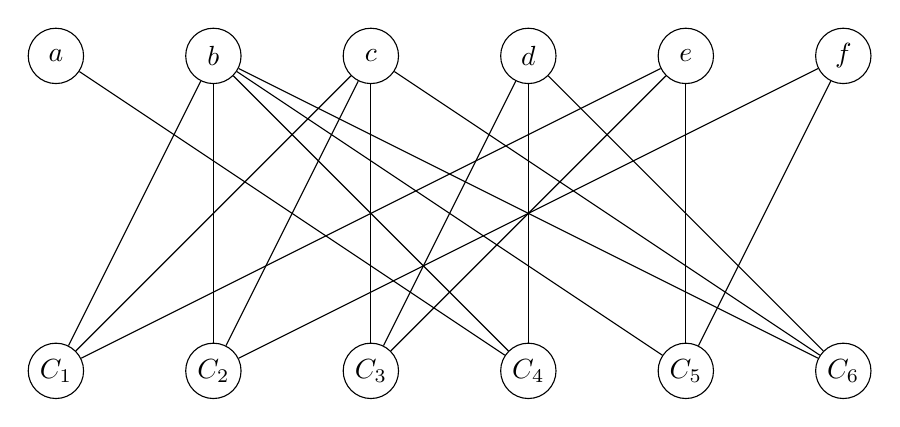
\begin{tikzpicture}
	\begin{scope}[auto, every node/.style={draw,circle,minimum size=2em,inner sep=1},node distance=2cm]
		\node[shape=circle,draw=black] (a) at (0,4) {$a$};
		\node[shape=circle,draw=black] (b) at (2,4) {$b$};
		\node[shape=circle,draw=black] (c) at (4,4) {$c$};
		\node[shape=circle,draw=black] (d) at (6,4) {$d$};
		\node[shape=circle,draw=black] (e) at (8,4) {$e$};
		\node[shape=circle,draw=black] (f) at (10,4) {$f$};
		\node[shape=circle,draw=black] (1) at (0,0) {$C_1$};
		\node[shape=circle,draw=black] (2) at (2,0) {$C_2$};
		\node[shape=circle,draw=black] (3) at (4,0) {$C_3$};
		\node[shape=circle,draw=black] (4) at (6,0) {$C_4$};
		\node[shape=circle,draw=black] (5) at (8,0) {$C_5$};
		\node[shape=circle,draw=black] (6) at (10,0) {$C_6$};
	\end{scope}
	\path [-](1) edge node {} (b);
	\path [-](1) edge node {} (c);
	\path [-](1) edge node {} (e);
	\path [-](2) edge node {} (b);
	\path [-](2) edge node {} (c);
	\path [-](2) edge node {} (f);
	\path [-](3) edge node {} (c);
	\path [-](3) edge node {} (d);
	\path [-](3) edge node {} (e);
	\path [-](4) edge node {} (a);
	\path [-](4) edge node {} (b);
	\path [-](4) edge node {} (d);
	\path [-](5) edge node {} (b);
	\path [-](5) edge node {} (e);
	\path [-](5) edge node {} (f);
	\path [-](6) edge node {} (b);
	\path [-](6) edge node {} (c);
	\path [-](6) edge node {} (d);
	
	\end{tikzpicture}
	\caption{Example preliminary graph $G_A$ on $\phi$}
	\label{fig:ga}
\end{figure}

\begin{figure}[h] 
		\captionsetup{justification=centering}
		
		\centering 
		\begin{tikzpicture}
		\begin{scope}[auto, every node/.style={draw,circle,minimum size=2em,inner sep=1},node distance=2cm]
			\node[shape=circle,draw=black] (b) at (0,4) {$b_T$};
			\node[shape=circle,draw=black] (bb) at (2,4) {$b_F$};
			\node[shape=circle,draw=black] (c) at (4,4) {$c_T$};
			\node[shape=circle,draw=black] (cc) at (6,4) {$c_F$};
			\node[shape=circle,draw=black] (e) at (8,4) {$e_T$};
			\node[shape=circle,draw=black] (ee) at (10,4) {$e_F$};
			\node[shape=circle,draw=black] (f) at (12,4) {$f_T$};
			\node[shape=circle,draw=black] (ff) at (14,4) {$f_F$};
			
			\node[shape=circle,draw=black] (1) at (0,0) {$C_1^1$};
			\node[shape=circle,draw=black] (2) at (2,0) {$C_1^2$};
			\node[shape=circle,draw=black] (3) at (4,0) {$C_1^3$};
			\node[shape=circle,draw=black] (4) at (6,0) {$C_1^4$};
			\node[shape=circle,draw=black] (5) at (8,0) {$C_2^1$};
			\node[shape=circle,draw=black] (6) at (10,0) {$C_2^2$};
			\node[shape=circle,draw=black] (7) at (12,0) {$C_2^3$};
			\node[shape=circle,draw=black] (8) at (14,0) {$C_2^4$};
		\end{scope}
		\path [-](1) edge node {} (bb);
		\path [-](1) edge node {} (cc);
		\path [-](1) edge node {} (ee);
		\path [-](2) edge node {} (b);
		\path [-](2) edge node {} (c);
		\path [-](2) edge node {} (ee);
		\path [-](3) edge node {} (b);
		\path [-](3) edge node {} (cc);
		\path [-](3) edge node {} (e);
		\path [-](4) edge node {} (bb);
		\path [-](4) edge node {} (c);
		\path [-](4) edge node {} (ee);
		\begin{scope}[>={Stealth[black]},
		every edge/.style={draw=red}]
		\path [-](5) edge node {} (bb);
		\path [-](5) edge node {} (cc);
		\path [-](5) edge node {} (ff);
		\path [-](6) edge node {} (b);
		\path [-](6) edge node {} (c);
		\path [-](6) edge node {} (ff);
		\path [-](7) edge node {} (b);
		\path [-](7) edge node {} (cc);
		\path [-](7) edge node {} (f);
		\path [-](8) edge node {} (bb);
		\path [-](8) edge node {} (c);
		\path [-](8) edge node {} (ff);
		\end{scope}   
		\end{tikzpicture}
	\caption{Snippet of example final graph $G_B$ on $\phi$.}{Only $C_1$ and $C_2$ is shown}
	\label{fig:gb}
\end{figure}

Professor Dawar's construction creates rigid graphs based off the $odd$ property of multipedes. The oddness property is replaced with check for unique satisfiability of an 3-XOR-Formula. Similarly the check for $k$-local consistency is replaced by identifying whether 3-XOR-Forumlas are solved quicker using Gaussian elimination operating within the algorithm, in comparison to the same formula without Gaussian elimination. In short, the check for oddness is replaced by unique satisfiability, thereby rendering them rigid, and the check for $k$-local consistency is estimated by comparing Gaussian elimination on and off times.

\newpage
\section[Solvers]{Solvers}
In order to construct our graphs, we will require multiple checks at different stages of construction. When we generate a random 3-XOR-Formula $\phi$, we need to ensure that it is $k$-locally consistent, uniquely satisfiable and gives rise to a preliminary graph with no automorphisms.  Checking for $k$-local consistency and unique satisfiability requires a SAT solving program to determine these attributes. Whereas a GI solver, namely Traces, is utilised to check for automorphisms.

\subsection[GI Solvers]{GI Solvers}
The programs Nauty and Traces are two of the fastest GI solvers for most cases of small and large graphs respectively. Nauty  was developed in the 1980s by B. Mckay \cite{mckay1981practical}, which was subsequently revised and incorporated into Traces \cite{mckay2014practical} in 2013. These programs utilise two key components in their algorithms: vertex colour refinement and factoring of graphs through found automorphisms.

Two main procedures provided by the Nauty and Traces are Automorphism Group ($Aut(G)$) and Canonical Labelling ($Canon(G)$) of graphs. Our work is concerned only with the $Aut(G)$ function, as graphs which execute slowly on $Aut(G)$ tend execute slowly on Canon(G) \cite{mckay2014practical}. These procedures are used to benchmark the performance of their algorithm, since the exact complexity of these programs is unknown. Additionally, since $Aut(G)$ shows us whether there are any automorphisms of a graph G, we use this feature in validating our preliminary graph $G_A$, as well as determining the performance of our final graph $G_B$.

The heuristic algorithm behind Nauty and Traces to determine graph isomorphism is a backtracking search which is based off two key elements: vertex colour refinement (also known as a 1-dimensional Weisfeiler-Leman test) and factoring graphs through found automorphisms \cite{mckay2014practical}. Our construction, being both rigid and resistant to Weisfeiler-Leman tests and its high dimensional variants, should be difficult for this algorithm.

\newpage
\subsection{SAT Solvers}
The algorithms behind SAT solvers typically use Gaussian Elimination in solving a system of linear equations. In some cases, this feature can be disabled, and some implementations do not use it all. By toggling Gaussian Elimination on and off, and recording the times, one can make a good guess at whether $\phi$ is $k$-locally consistent. Randomly generated systems which are solved significantly faster with Gaussian Elimination on versus off are ones of interest. The prediction is that systems with greater differences in execution speeds hints at $k$-local consistency of a system.

\section{Previous Attempt}
Recently, a study searched for the family of graphs Babai describes. E. Arrighi, a Cambridge intern guided by Prof. A. Dawar, the project supervisor, found that multipedes are theoretically complex for Traces. Arrighi concluded that the smallest examples of suitable probabilistically generated multipedes, containing significantly high probability of non-trivial automorphisms, would be too large to generate, so rendering them too large for experimentation on Traces. Instead, our approach utilised the same concepts from such hypergraphs, but constructs them in a smaller fashion.








